% ============================================================
%  CHAPTER 2 — Project Management
% ============================================================

\chapter{Project Management}

% ──────────────────────────────────────────
\section{Introduction}
% ──────────────────────────────────────────

This chapter presents the organizational aspects of the project carried
out during my internship. It describes the methods, tools, and practices
used to structure the work, improve collaboration, and ensure efficient
task completion.

Effective project organization is an essential factor in the success of
any technical project. It allows teams to collaborate smoothly,
communicate clearly, and deliver high-quality results within the expected
timeframe. Throughout this chapter, the internship process, the project
management tools, the adopted methodology, and the project planning are
presented.

% ──────────────────────────────────────────
\section{Internship Process}
% ──────────────────────────────────────────

This section describes the main phases of my internship at Oracle, from
the onboarding period to the technical training.

  % ── 2.2.1 ──
  \subsection{Onboarding Phase}

  The initial phase of my internship at Oracle consisted of becoming
  familiar with the company's internal environment and the Morocco
  Research and Development Center (MADC). This phase included meetings
  with key people, such as the HR manager, the program manager, members
  of the Oracle Morocco team, my mentor, and the project team.

  During this period, I also received my internship equipment and
  participated in introductory sessions that helped me understand the
  objectives of the project, the team organization, and the expectations
  related to my work. After receiving my workstation, I configured the
  required working environment, including SSO, VPN, and BitLocker.

  \begin{figure}[h]
    \centering
    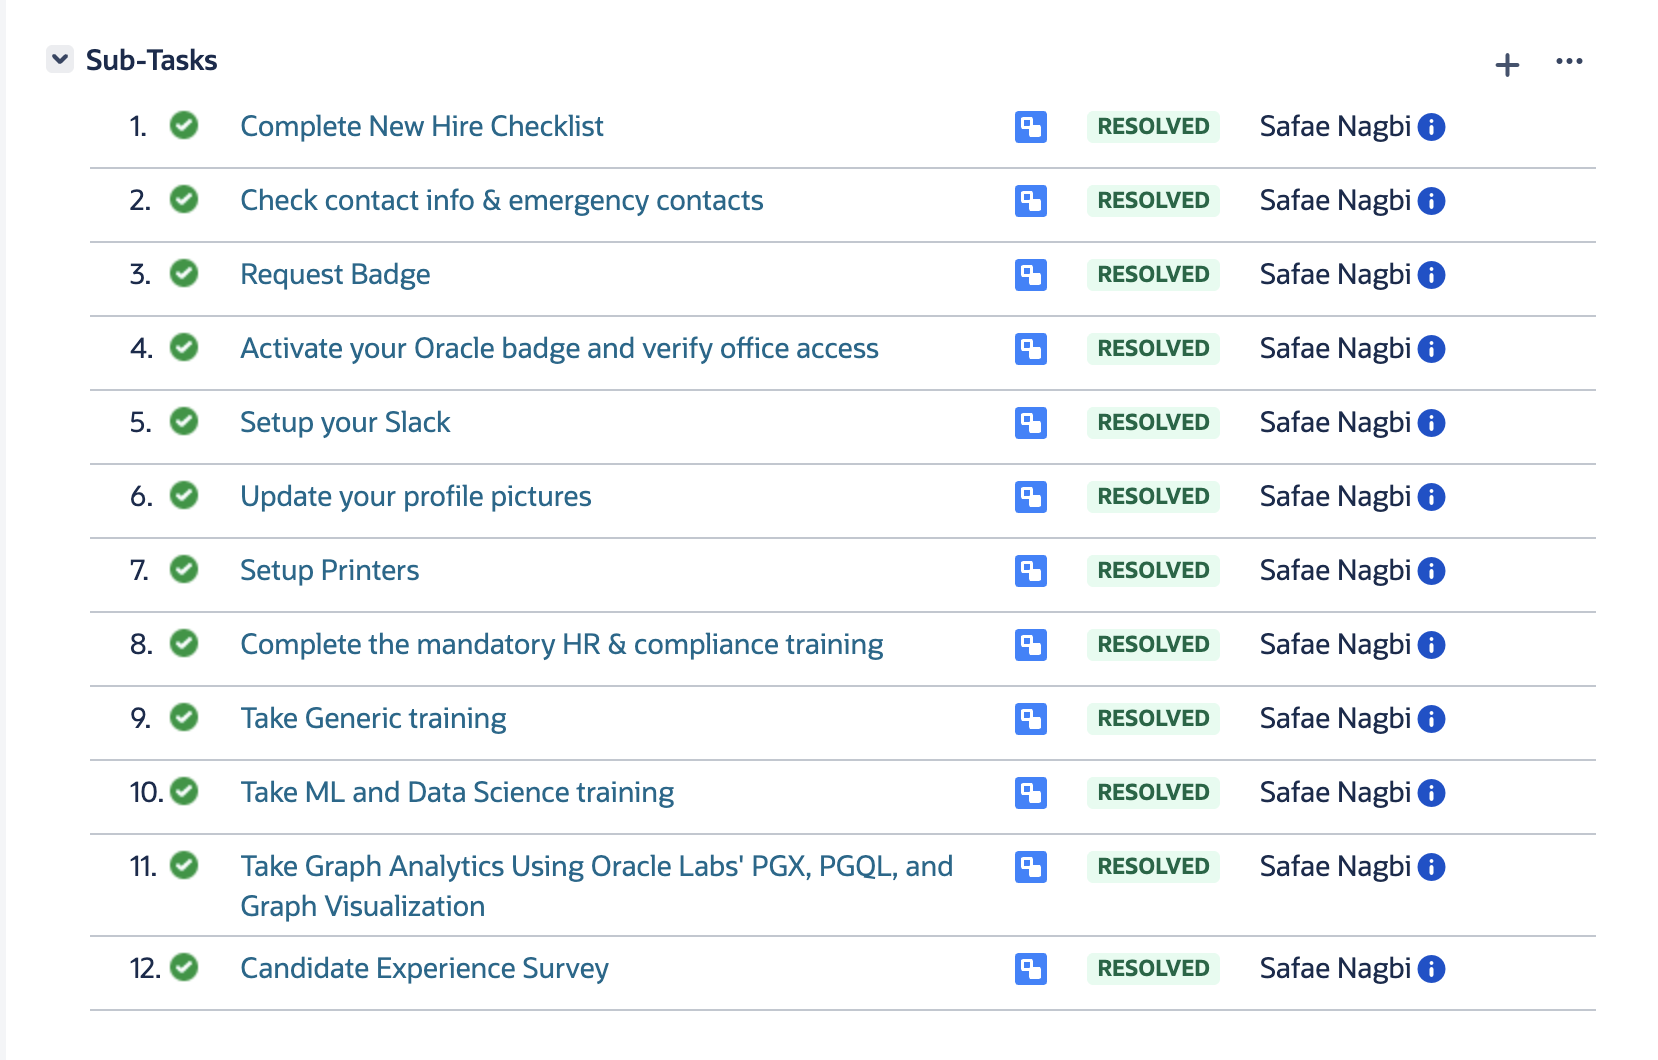
\includegraphics[width=0.8\textwidth]{figures/jira_ticket_example}
    \caption{Jira Ticket Example}
    \label{fig:jira_ticket_example}
  \end{figure}

  % ── 2.2.2 ──
  \subsection{Training Phase}

  I completed a comprehensive compliance training program covering
  essential company policies, security rules, and internal regulations.
  This training provided a solid foundation for the internship and helped
  ensure that I was aware of my responsibilities and Oracle's
  expectations.

  Following this compliance training, I started a series of generic
  technical training sessions focused on strengthening my foundations in
  several areas, including Oracle Cloud Infrastructure (OCI), DevOps, and
  Linux.

  \begin{figure}[h]
    \centering
    %\includegraphics[width=0.8\textwidth]{figures/generic_training}
    \fbox{\parbox{0.8\textwidth}{\centering Placeholder for Generic Training figure}}
    \caption{Generic Training}
    \label{fig:generic_training}
  \end{figure}

  Once the foundational training sessions were completed, I moved on to
  more specific training related to the project requirements. This
  included APEX foundations and the development of small applications in
  order to practice and better understand the tools used within the team.

% ──────────────────────────────────────────
\section{Management Tools}
% ──────────────────────────────────────────

To facilitate collaboration, communication, documentation, and task
tracking, several management tools were used throughout the internship.
The main tools are presented in the following sections.

  % ── 2.3.1 ──
  \subsection{Confluence}

  Confluence provided a centralized platform for knowledge sharing and
  documentation. It was used to document tasks, research, technical
  notes, and project-related information throughout the internship.
  It also served as a repository where useful project details and
  references could be stored and accessed by the team~\cite{confluence}.

  % ── 2.3.2 ──
  \subsection{Zoom}

  Zoom was used as a video conferencing platform to participate in
  virtual meetings with the team. It offered a practical and efficient
  solution for remote communication and collaboration, allowing clear
  discussions and regular follow-up meetings~\cite{zoom}.

  % ── 2.3.3 ──
  \subsection{Jira}

  Jira, a project management and issue-tracking tool developed by
  Atlassian, was used to organize tasks, track progress, assign work,
  set priorities, and manage project workflows. It allowed the team to
  follow the status of different tasks and ensure that deadlines were
  respected.

  Jira supports several project management methodologies, including
  Agile, Scrum, and Kanban. It provides features such as boards,
  backlogs, issues, and sprints, which helped structure the work and
  monitor progress throughout the internship~\cite{jira}.

  % ── 2.3.4 ──
  \subsection{Slack}

  Slack was used as a centralized communication hub for the team. It
  enabled real-time information sharing, discussions about project
  updates, direct messaging, and file sharing. Its channel-based
  organization helped keep conversations structured and accessible.

  In addition, the search functionality in Slack channels was
  particularly useful for debugging and problem solving. It made it
  possible to quickly retrieve previous discussions or similar internal
  errors shared by other team members, which saved significant time
  during development~\cite{slack}.

% ──────────────────────────────────────────
\section{Project Methodology}
% ──────────────────────────────────────────

Throughout the internship, the team followed the Scrum framework, which
is one of the most widely used frameworks within Agile methodology.
Scrum helped structure the project into iterative development cycles,
allowing the team to adapt to changing requirements while maintaining a
clear focus on delivering valuable increments.

To illustrate this methodology, consider the example of building a
simple to-do list application. If the product owner prioritizes two
features for the first sprint, such as adding new tasks and marking tasks
as completed, the team focuses on implementing these features during the
sprint. During development, team members review each other's work and
test the features to verify that they meet the acceptance criteria
defined at the beginning. At the end of the sprint, a functional
increment of the application is delivered.

In this project, the product backlog was prioritized according to the
value and relevance of the tasks. Since some requirements were still
evolving and could change over time, Scrum was an appropriate approach.
It supported flexibility, continuous feedback, and progressive
improvement.

Furthermore, the Scrum framework encouraged communication,
collaboration, and continuous improvement. By following Agile principles,
the team was able to respond to change, iterate quickly, and work toward
a high-quality solution aligned with stakeholder expectations.

The main Agile principles followed during the project are:

\begin{enumerate}
  \item Customer satisfaction through early and continuous delivery of
  valuable software.

  \item Welcoming changing requirements, even late in development, in
  order to support the customer's competitive advantage.

  \item Delivering working software frequently, with a preference for
  shorter timescales.

  \item Maintaining collaboration between business stakeholders and
  developers throughout the project.

  \item Building projects around motivated individuals by giving them the
  environment and support they need and trusting them to get the job done.

  \item Prioritizing face-to-face conversation as an efficient and
  effective method of communication within the development team.

  \item Considering working software as the primary measure of progress.

  \item Promoting sustainable development so that sponsors, developers,
  and users can maintain a constant pace.

  \item Maintaining continuous attention to technical excellence and good
  design.

  \item Valuing simplicity, which means maximizing the amount of work not
  done.

  \item Allowing the best architectures, requirements, and designs to
  emerge from self-organizing teams.

  \item Reflecting regularly on how to become more effective, then
  adjusting the team's behavior accordingly~\cite{agile}.
\end{enumerate}

\begin{figure}[h]
  \centering
  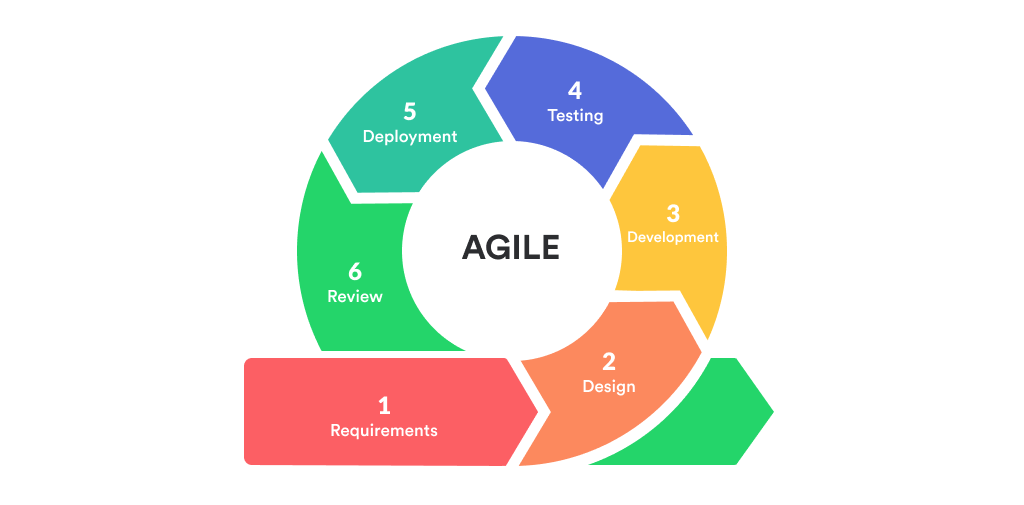
\includegraphics[width=0.8\textwidth]{figures/agile_methodology}
  \caption{Agile Methodology}
  \label{fig:agile_methodology}
\end{figure}

In my case, I also had additional meetings with different team members.
These meetings were mainly opportunities to discuss tasks in more detail,
clarify technical points, and follow the progress of the work.

% ──────────────────────────────────────────
\section{Gantt Chart}
% ──────────────────────────────────────────

A Gantt chart, named after its creator Henry L. Gantt, is a visual tool
used in project management to represent tasks along a timeline. It uses
horizontal bars to show the duration of each task, the dependencies
between tasks, and the overall schedule of a project.

This tool makes complex project planning easier to understand by
presenting tasks, milestones, and deadlines in a clear visual format. It
helps project managers and team members monitor progress, identify
delays, and keep the project aligned with its expected timeline.

In the context of this internship, the Gantt chart summarizes the main
phases of the project during the first four months, from the onboarding
process to the writing of this report.

\begin{figure}[h]
  \centering
  %\includegraphics[width=0.9\textwidth]{figures/gantt_chart}
  \fbox{\parbox{0.9\textwidth}{\centering Placeholder for Gantt Chart}}
  \caption{Gantt Chart}
  \label{fig:gantt_chart}
\end{figure}

% ──────────────────────────────────────────
\section{Conclusion}
% ──────────────────────────────────────────

This chapter presented the organizational dimensions of the project. It
described the internship process, including onboarding and training, as
well as the tools used to support communication, documentation, and task
management.

The chapter also introduced the Scrum methodology adopted during the
project and explained how Agile principles helped structure the work and
support collaboration. Finally, the Gantt chart provided an overview of
the project timeline. These organizational elements contributed to a
clearer workflow and helped ensure the successful progress of the
internship project.